% ANTUMBRA whitepaper, English edition, version 1.2.
% Bitcoin-style layout: no cover page, title block on page 1, abstract,
% contents, then numbered sections. Black and white only.
\documentclass[11pt,a4paper]{article}

\usepackage[T1]{fontenc}
\usepackage{amsmath}
\usepackage{newtxtext,newtxmath}
\usepackage{geometry}
\geometry{a4paper, top=2.6cm, bottom=2.6cm, left=2.5cm, right=2.5cm}
\usepackage{graphicx}
\usepackage{booktabs}
\usepackage{tabularx}
\newcolumntype{Y}{>{\raggedright\arraybackslash}X}
\newcolumntype{L}[1]{>{\raggedright\arraybackslash}p{#1}}
\usepackage{enumitem}
\usepackage{titlesec}
\usepackage{microtype}
\usepackage{tikz}
\usetikzlibrary{arrows.meta,positioning}
\usepackage[hidelinks,bookmarks=true,bookmarksnumbered=true,unicode=true]{hyperref}

% typography discipline
\widowpenalty=10000
\clubpenalty=10000
\setlength{\parskip}{2.5pt plus 1pt}

% section spacing, plain and quiet
\titleformat{\section}{\large\bfseries}{\thesection}{0.7em}{}
\titlespacing*{\section}{0pt}{14pt plus 4pt minus 2pt}{6pt}
\titleformat{\subsection}{\normalsize\bfseries}{\thesubsection}{0.6em}{}
\titlespacing*{\subsection}{0pt}{10pt plus 3pt minus 2pt}{4pt}

\hypersetup{
  pdftitle={ANTUMBRA: A Reputation-Anchored Settlement Network for the Human-Machine Economy},
  pdfauthor={XelisVault},
  pdfsubject={Blockchain protocol specification},
  pdfkeywords={ANTUMBRA, ATU, blockchain, privacy, reputation, BlockDAG, RandomX, CryptoNote, AI governance}
}

\begin{document}

% ── title block, in the manner of a classical whitepaper ──
\begin{center}
  {\LARGE\bfseries ANTUMBRA}\\[9pt]
  {\large A Reputation-Anchored Settlement Network\\for the Human-Machine Economy}\\[9pt]
  {\normalsize XelisVault}\\[2pt]
  {\small\ttfamily xelisvault.xyz \; $\cdot$ \; github.com/XelisVault/Antumbra}\\[2pt]
  {\small Version 1.2, September 2026}
\end{center}

\vspace{10pt}

\begin{abstract}
\noindent
ANTUMBRA is a settlement network built for a problem that no existing chain
treats as a protocol primitive: verifiable trust between humans and machines.
Millions of software agents already buy, sell and pay on behalf of people,
over rails built on fully transparent stablecoins; those rails say nothing
about whether an agent is reliable, who answers for it, or where its budget
ends. Dominant proofs of humanity engrave body data into global registries,
and the coins that are actually private remain slow or unreadable to
regulators. ANTUMBRA aims at that square: no deployed chain combines the
five properties it requires, and each of the nearest neighbors renounces at
least two. It couples a CPU-mined BlockDAG with two-second blocks and
private-by-default transactions, a finality committee of fifty-five seats
drawn by reputation rather than capital, non-biometric human identities,
agents that are accountable by construction, and a native three-level
disclosure mechanism. The scarce resource the network mints is consensus
reputation, Kleos: three layers of which the heaviest is time itself, which
cannot be bought. Above the whole, a machine governance layer, the Corona,
lets AI senators propose, red-team and implement protocol changes under
human veto, paid like miners for useful work and ruined like miners for
attacks. The money supply is capped at 16,180,339 ATU, the golden ratio
scaled by ten million, issued over thirty-four four-year eclipses and closed
exactly at year 136. The specification was attacked by its own deterministic
simulation before being written down as final: one flaw was found and four
corrective rules closed it, the engine is public code, and the rules hold on
a sweep of twelve seeds. A first external audit of version 1.1 returned
twelve findings; this version closes them. This document is the public
reference specification for the network.
\end{abstract}

\vspace{4pt}
\tableofcontents
\vspace{4pt}

% Sections 1 to 3.

\section{Introduction}\label{sec:intro}

A blockchain earns its existence only by serving a structural, growing and
badly served demand. Four currents converge in 2026 on the same point, and
no deployed chain occupies it: the nearest neighbors, reviewed in
Table~\ref{tab:neighbors}, each renounce at least two of its requirements.
The first is agent commerce. Coinbase revived HTTP status code 402 with the
x402 protocol, Stripe and Coinbase contest the machine-to-machine payment
rails, and four rival standards share the same territory. All of these rails
share three blind spots: they are denominated in stablecoins, they are fully
transparent, and they carry no portable trust. An agent pays on them;
nothing says whether it is reliable, for whom it acts, or who answers for
it. Yet a merchant cashing out an unknown agent, an accountant auditing a
fleet of agents, and a client delegating a budget all need the same thing:
to know who they are dealing with.

The second current is proof of humanity. Bots saturate the web to the point
that platform defense has become the separation of persons from programs.
The dominant answers are biometric: iris scans for one project, biometry
woven into consensus for another. Each accumulates the same debt, a body
measurement that is irreversible, centralized at collection even when the
proof is decentralized. Once an iris template is engraved somewhere, there
is no second chance; the perfect registry of future leaks is already
written. The third current is regulatory. MiCA and the FATF Travel Rule
keep sustained pressure on private coins, while Zcash demonstrates the
practicable path: a regulator who looks at its mechanism understands it,
shielded pools, viewing keys, explicit disclosure. Readability, not
transparency, is the acceptance criterion. The fourth current is
instantaneity. A counter payment must become irreversible in seconds; the
existing private chains require tens of seconds to minutes of real
finality.

\begin{table}[htbp]
\centering
\small
\caption{The four demands of 2026 and the empty square at the center.}
\label{tab:demands}
\begin{tabularx}{\textwidth}{@{}L{4.1cm}YY@{}}
\toprule
Demand in 2026 & Dominant offer & Blind spot left open \\
\midrule
Agent payments (x402, MPP, ACP, AP2) & HTTP rails on transparent stablecoins &
portable trust, privacy, a designated answerable party: none \\
Proof of humanity & biometrics (iris, face, veins) &
non-biometric personhood, with no body registry \\
Sustainable privacy (MiCA, Travel Rule) & Zcash: selective disclosure; Monero: opacity &
native privacy with provable compliance \\
Quasi-instant private payment & Kaspa (fast, transparent); Monero (private, slow) &
fast, private, finalized in seconds, on egalitarian hardware \\
\bottomrule
\end{tabularx}
\end{table}

\begin{table}[htbp]
\centering
\small
\caption{The neighbors of the square, and what each renounces. The
reference here is honest: rings and fast DAG ordering are inherited arts,
not inventions of this paper.}
\label{tab:neighbors}
\begin{tabularx}{\textwidth}{@{}L{3.2cm}Y Y@{}}
\toprule
Chain & Closest strength & What it renounces of the five properties \\
\midrule
Monero, NERVA & the reference of private payment & speed (minutes of finality), agent identity, disclosure levels \\
Zcash (Orchard) & readable selective disclosure & egalitarian CPU mining (Equihash ASIC territory), agent identity, speed \\
Kaspa & fast DAG ordering at scale & privacy entirely, disclosure, reputation \\
Xelis & encrypted amounts on a DAG & ring anonymity (no decoys), reputation, CPU-only mining \\
Penumbra, Namada & shielded multi-asset, ZK disclosure & CPU mining, egalitarian hardware, reputation as consensus \\
Aztec, Aleo & private general computation & every proof circuit is maximal technique and maximal audit surface; CPU mining \\
ANTUMBRA & the five properties together & general masked contracts, honestly deferred (Section~\ref{sec:contracts}) \\
\bottomrule
\end{tabularx}
\end{table}

The center of Table~\ref{tab:demands} is empty, and not for technical
reasons. It is empty because each ecosystem optimized a single dimension:
agent rails optimized throughput, biometrics optimized anti-sybil, Zcash
optimized regulatory legitimacy, Kaspa optimized speed. None of them treats
trust, meaning who acts, since when, answerable up to which human, as a
primitive of the protocol. The network that installs trust there must
combine five properties usually considered incompatible: speed, privacy by
default, provable disclosure, processor egalitarianism, and a reputation
that capital cannot fabricate. The thesis of this paper is that these
properties reinforce one another as soon as one of them, reputation
anchored in time, is treated as the foundation.

The monetary and consensus numbers that recur throughout this document are
gathered here for reference. Each is justified in the section indicated.

\begin{table}[htbp]
\centering
\small
\caption{Reference magnitudes of the network.}
\label{tab:magnitudes}
\begin{tabularx}{\textwidth}{@{}L{3.6cm}L{4.4cm}Y@{}}
\toprule
Quantity & Value & Meaning \\
\midrule
Monetary cap & 16,180,339 ATU & the golden ratio scaled by ten million; the same proportion already drives RandomX \\
Emission & 34 eclipses of 4 years & each eclipse emits 61.8\,\% of the previous one; the cap is reached exactly at year 136 \\
Blocks & 2 seconds & near-immediate inclusion; the DAG absorbs parallel blocks \\
Economic finality & under 6 seconds & checkpoints signed by the Ring, quorum of 37 out of 55 seats \\
Privacy & private by default & rings of sixteen, committed amounts, one-time addresses, Tor by default \\
Disclosure & selective, three levels & per transaction, per bounded auditor, per compliance proof \\
Reputation & Kleos, 0 to 100 & Deed 40, Echo 30, Tenure 30; non-transferable, corroded by time \\
Premine & 0\,\% & everything is mined or governed; nobody starts with an advantage \\
\bottomrule
\end{tabularx}
\end{table}

\section{Design Overview}\label{sec:overview}

ANTUMBRA separates cleanly what most chains pile up: settlement, finality,
identity and disclosure. The settlement layer, at the bottom, is a
CPU-mined BlockDAG that orders parallel blocks every two seconds and
carries private-by-default transactions: this is the Veil. The finality
layer, the Ring, is a committee of fifty-five high-reputation identities
that sign checkpoints every four seconds and make any payment irreversible
in under six seconds. The identity layer distinguishes humans, the Embers,
from agents, the Ciphers, with their admission and accountability rules.
The reputation layer, Kleos, feeds the Ring, locks sponsorships and weights
peer testimony. Around the whole, the Lumen, selective disclosure, forms
the ring of light that gives the network its name: a shadow faithfully
kept, proofs on demand.

\begin{figure}[htbp]
\centering
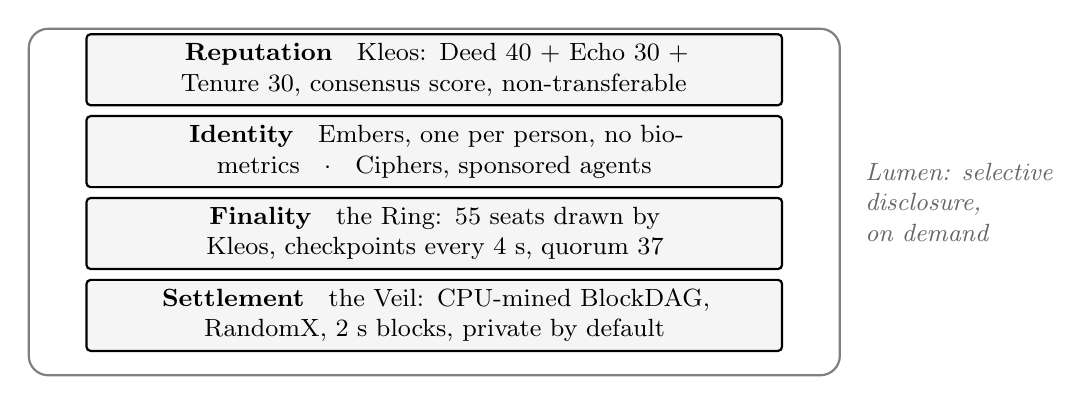
\begin{tikzpicture}[
  layer/.style={draw=black, thick, rounded corners=1.5pt, text width=8.6cm,
                minimum height=0.82cm, align=center, font=\small, fill=black!4},
]
  % Lumen enclosure
  \draw[rounded corners=7pt, thick, black!50]
        (-5.15,-0.78) rectangle (5.15,3.62);
  \node[anchor=west, font=\small\itshape, text=black!60, align=left]
        at (5.35,1.42) {Lumen: selective\\disclosure,\\on demand};
  % the four layers, top to bottom
  \node[layer] (rep) at (0,3.1)
    {\textbf{Reputation} \; Kleos: Deed 40 + Echo 30 + Tenure 30, consensus score, non-transferable};
  \node[layer] (ide) at (0,2.06)
    {\textbf{Identity} \; Embers, one per person, no biometrics \; $\cdot$ \; Ciphers, sponsored agents};
  \node[layer] (fin) at (0,1.02)
    {\textbf{Finality} \; the Ring: 55 seats drawn by Kleos, checkpoints every 4 s, quorum 37};
  \node[layer] (set) at (-0.0,-0.02)
    {\textbf{Settlement} \; the Veil: CPU-mined BlockDAG, RandomX, 2 s blocks, private by default};
\end{tikzpicture}
\caption{The four layers of ANTUMBRA inside the Lumen, the selective
disclosure ring. Each layer depends only on the layers below it.}
\label{fig:arch}
\end{figure}

The nomenclature is stable across the document; each name designates one
precise part and only one. The reader may return to Table~\ref{tab:naming}
at any time. The internal names are working codenames, chosen to keep the
document readable; they may be adapted at implementation time. Only
ANTUMBRA and its ticker ATU are proposed as a definitive commitment,
verified free of collision on the blockchain and crypto namespace on
September 6, 2026. One layer of Table~\ref{tab:naming} sits above the
others and outside the stack discipline: the Corona,
Section~\ref{sec:corona}, machine governance that reads every layer and
modifies none of them without the human chambers.

\begin{table}[htbp]
\centering
\small
\caption{Reference nomenclature.}
\label{tab:naming}
\begin{tabularx}{\textwidth}{@{}L{2.2cm}L{3.4cm}Y@{}}
\toprule
Name & Nature & Role in one sentence \\
\midrule
ANTUMBRA & the network & private settlement BlockDAG, CPU-mined \\
ATU & the currency & 16,180,339 units, divisible by $10^{8}$ \\
the Veil & privacy & rings of sixteen, committed amounts, one-time addresses, Tor by default \\
the Lumen & disclosure & hierarchical viewing keys and compliance proofs, on demand \\
the Ember & human identity & one per person, non-biometric, one vote in governance \\
the Cipher & agent identity & sponsored by an Ember, with a revocable spending perimeter \\
Kleos & reputation & three-layer score, consensus, non-transferable, non-purchasable \\
the Ring & finality committee & 55 high-reputation seats, checkpoints every 4 seconds \\
RAF & finality mechanism & Reputation-Anchored Finality \\
the Corona & machine governance & AI senators that propose, red-team and implement changes under human veto (Section~\ref{sec:corona}) \\
the Vault & deployment custody & threshold signature of 9 hardware fragments, 7 needed, no whole key anywhere \\
era & protocol time & six months; the unit of reputation, rotation and decay \\
eclipse & emission time & four years, eight eras; 34 eclipses lead to the cap at year 136 \\
Mandate & money contract & an output whose release obeys a predicate declared at creation \\
the Machine & logic contract & deterministic virtual machine on public state only, after genesis \\
\bottomrule
\end{tabularx}
\end{table}

Two principles govern the assembly. First, each layer depends only on the
layers below it: settlement ignores reputation, finality reads Kleos but
never writes it, identity builds on both without modifying either. That
stacking discipline is what keeps every part auditable in isolation and
replaceable without rewriting the rest. Second, the value loop: reputation
protects finality, finality makes payments instant, instant payments serve
agents and merchants, and their honorable behavior enriches reputation.
The network is designed so that its security and its utility feed each
other instead of taxing each other.

\section{The Settlement Layer: a CPU-Mined BlockDAG}\label{sec:settlement}

The first wager is egalitarian. RandomX, the algorithm designed so that one
ordinary computer is one vote, produces blocks that no specialized machine
produces better at equal cost: no dedicated circuit, no farm of graphics
cards. Miners run it in fast mode, 2,080 MiB of memory; verifying nodes
may run light mode, 256 MiB of cache and no dataset, a size its author
chose deliberately so that specialized hardware gains nothing by verifying:
the light-mode memory-time product was sized to close exactly that door.
Emission and block production stay within reach of anyone who owns
a laptop, the ethos of NERVA carried to its conclusion. The constant
\texttt{0x9E3779B9}, the integer truncation of the golden ratio in binary
arithmetic, already drives the generation of RandomX superscalar programs;
the same proportion that will distribute the currency already works inside
the engine that will mine it, a mnemonic accident the paper claims as
identity, not as argument.

The second wager is structural. A linear chain must choose between short
blocks, which multiply orphans, and long blocks, which slow confirmation;
a DAG orders parallel blocks instead of rejecting them. At a two-second
cadence, a linear proof-of-work network would lose an unsustainable share
of its blocks; a fast-converging DAG integrates them into its partial
order and accumulates the work of all of them. Speed stops being a
trade-off against egalitarianism: it becomes its product. The ordering
layer belongs to the GHOSTDAG family, whose public literature and existing
implementations provide the operational definitions of convergence and
anticone.

\begin{table}[htbp]
\centering
\small
\caption{Parameters of the settlement layer.}
\label{tab:settlement}
\begin{tabularx}{\textwidth}{@{}L{4.0cm}L{4.6cm}Y@{}}
\toprule
Parameter & Retained value & Justification \\
\midrule
Mining algorithm & RandomX: fast mode 2,080 MiB, light mode 256 MiB & proven by years of attack; the light-mode cache is sized so verification resists specialization \\
Block cadence & 2 seconds & near-immediate inclusion; the DAG absorbs the orphan rate \\
Block ordering & GHOSTDAG-family coloring, cluster parameter $k = 8$ & security grows with block volume, not only depth; $k$ is calibrated for the two-second cadence \\
Flow anonymity & ring of 16, masked amounts & equals the strongest ring deployed in the lineage (Monero since 2022); a floor to raise, not a ceiling \\
Signature scheme & MLSAG over Ed25519, Keccak-256 & the lineage construction, implemented and cross-validated; CLSAG is the post-audit upgrade candidate \\
Transport network & Dandelion++, Tor for transaction injection & IP-address analysis is the number one practical flaw of private chains \\
Finality & Ring checkpoints (Section~\ref{sec:ring}) & economic irreversibility in under 6 seconds \\
Target throughput & 100 tx/s sustained, 300 tx/s burst, on the reference node & an engineering budget with a measured exit criterion (Table~\ref{tab:capacity}) \\
Storage & pruned DAG, decoy pool retained forever & the nullifier set and output keys are consensus data; the growth budget is stated in Table~\ref{tab:capacity} \\
\bottomrule
\end{tabularx}
\end{table}

Pruning deserves its own paragraph, because it conditions the entire social
contract, and in a ring chain it is not free: spent outputs remain decoys
for everyone else's privacy, so the output keys, their commitments and the
nullifier set are consensus data forever, roughly ninety-six bytes per
output. What prunes is the rest: the ring signatures, the range proofs and
the transaction bodies beyond the recent window, which no later
verification re-reads. A network whose nodes required a disk bay would
exclude exactly the participants it claims to serve; the growth budget of
Table~\ref{tab:capacity} keeps that promise measurable. Dandelion++ stem
propagation and Tor transport close the door on IP-address analysis, which
remains the great practical weakness of badly configured private networks:
transactional privacy is nothing if the network observer knows who emitted
what. One precision, because latency and a DAG interact: transactions are
injected through Tor, but blocks relay node to node over the peer network
with mandatory encryption, so the stem anonymity of a payment never slows
the ordering of blocks that carry it, and the cluster parameter $k$ is
calibrated against measured propagation at the two-second cadence, an exit
criterion of the prototype phase, not an assumption.

\subsection{The DAG contract, stated precisely}

A specification that grafts rings onto a DAG must say exactly where the
seams are. The rules, frozen here and implemented in the reference node:
\begin{enumerate}[leftmargin=1.7em, itemsep=3pt, topsep=4pt]
\item \textbf{Ordering.} The coloring is GHOSTDAG-family with cluster
parameter $k = 8$: a block is blue when its anticone in the selected
parent's past is at most $k$; the blue score accumulates, the selected
parent maximizes it, and the consensus order is the depth-first walk of the
selected-parent chain absorbing blue blocks, then the remaining red blocks
in insertion order. Deterministic in the accepted set alone.
\item \textbf{Validity resolves in consensus order, not arrival order.} A
double spend published in parallel blocks is resolved by the order: the
first occurrence in consensus order spends the output, every later
occurrence is rejected at ordering time. The nullifier registry, the set of
published key images, is keyed by this order, so two conflicting
transactions in one anticone have exactly one winner, decided by a rule
every node recomputes identically.
\item \textbf{Decoys are drawn from the ordered past.} A wallet samples
decoys only from outputs already ordered by the DAG, never from the
anticone: an unordered output may yet be a parallel spend, and a decoy that
could become invalid is a decoy that betrays the real signer. Age brackets
follow the real spending distribution, the lineage's known discipline.
\item \textbf{Scanning.} Every output carries a one-byte view tag derived
from the shared secret: a wallet skips the full elliptic-curve derivation
for the outputs the tag does not match, so scanning stays linear and cheap
at any block cadence.
\item \textbf{Pruning.} Output keys, commitments, encrypted amounts and
nullifiers are retained forever; signatures, range proofs and bodies prune
after the verification window. Archival nodes keep everything by choice,
never by obligation.
\end{enumerate}

\subsection{The capacity budget, stated as numbers}

A private network that claims a throughput must show its arithmetic,
because privacy is precisely what makes verification expensive. The
reference node is a 2020-class desktop, four cores and eight gibibytes.
One standard transfer, two inputs and two outputs at ring sixteen,
verifies in about ten milliseconds of single-core work, dominated by the
MLSAG chains and the aggregated range proof; four cores therefore clear on
the order of four hundred transactions per second of pure verification,
before memory and bandwidth contend. The budget below is the honest form
of the claim: targets are what the exit criteria measure on the prototype
network, and the sustained expectation of a payment network of this size
is five to twenty transactions per second for the first years; the hundred
is headroom against spikes, not a promise of volume.

\begin{table}[htbp]
\centering
\small
\caption{The capacity budget of the reference node (4 cores, 8 GiB), and
what each target commits to.}
\label{tab:capacity}
\begin{tabularx}{\textwidth}{@{}L{3.1cm}Y Y@{}}
\toprule
Resource & Budget & Consequence \\
\midrule
Verification & $\sim$10 ms per tx, single core; 4 cores in parallel & the phase-1 exit criterion: 100 tx/s sustained for 24 h on the reference node \\
Bandwidth & $\sim$1.5 kB per tx, $\sim$1.5 Mbit/s sustained; 4.5 Mbit/s at burst & fits any residential connection; measured on the prototype, not asserted \\
Decoy pool growth & $\sim$192 B per tx: 56 GiB per year at 10 tx/s, 564 GiB if 100 tx/s were held for a year & the ceiling is burst capacity, not a promise; at the sustained expectation a one-terabyte disk holds the pool for a decade \\
Pruned node body & signatures and proofs beyond the window pruned & the 1 TiB disk also holds the recent bodies with ample margin \\
Burst ceiling & 300 tx/s for minutes on 8-core hardware & validated on the test network before phase five, or the sustained target drops \\
\bottomrule
\end{tabularx}
\end{table}

One honest word to close the section: grafting a fast-converging DAG onto
a CryptoNote base is a real engineering challenge, work of substance and
not a configuration flag. The roadmap (Section~\ref{sec:roadmap}) treats
it as the first technical risk of the project, with an isolated prototype
and a dedicated audit before any main network. The rules above make the
seam precise: cluster parameter, order resolution, decoy sampling,
scanning and pruning are stated, implemented and cross-validated, the
literature is public and solid, and none of the primitives used is exotic:
the risk is a degree of difficulty, not a degree of uncertainty.

% Sections 4 to 6.

\section{The Life Cycle of a Transaction}\label{sec:tx}

This section describes what lives on the network and how payments work,
step by step, from the composition of a payment in the wallet to its
irreversibility. A private transaction worthy of the name must prove four
things without revealing anything: that the sender owned the funds, that
the amounts balance, that the coin being spent was never spent elsewhere,
and that the sender authorized the spending. Each proof rests on a
distinct cryptographic construction, inherited from the CryptoNote lineage
that Monero and NERVA have carried for a decade and validated under
continuous attack. The merit of that lineage is not the invention of
exotic objects: it is the composition of simple, individually proven
objects into a system whose privacy property is demonstrable rather than
declared.

\subsection{Step 1: the one-time address}

Every payment identity publishes two public keys, a viewing key $A$ and a
spending key $B$. When Alice pays Bob, she draws a random value $r$,
computes the point $R = rG$, then derives a one-time destination address
$P$ that nobody can link to Bob's published address. Bob scans every new
output of the DAG and recognizes his own by replaying the same computation
with his private viewing key $a$: one multiplication and one addition
suffice, and a wallet can scan thousands of outputs per second. Each
output also carries a one-byte view tag, the top byte of the shared
secret: for the outputs whose tag does not match, Bob's wallet skips the
curve derivation entirely, so scanning stays linear and cheap at a
two-second cadence. No address is ever reused; graph analysis, the first
weapon of transparent chains, has no node to hold on to.
\begin{equation}\label{eq:onetim}
P = H_s(rA)\,G + B
\qquad\text{and, on the recipient side,}\qquad
P = H_s(aR)\,G + B
\end{equation}
with $R = rG$ published in the transaction, $H_s$ a hash mapped onto the
curve, and $G$ the group generator.

\subsection{Step 2: amounts under commitment}

The amount $v$ of each output is never written in clear. It is sealed in
a Pedersen commitment: an envelope with a remarkable property, addition.
Two envelopes can be summed, and their sum commits to the sum of the
amounts, without anyone opening the envelopes. That homomorphy lets the
network verify conservation of amounts at every spend while remaining
unable to read a single amount. The blinding factor $b$, specific to each
output, forbids the brute-force guessing of small amounts, the historical
weakness of the first masked currencies; it also ties the output to its
recipient, who alone can reconstruct its value.
\begin{equation}\label{eq:pedersen}
C = vH + bG
\end{equation}

\subsection{Step 3: the ring of decoys}

A spend references prior outputs; referencing them directly would reveal
the graph. The ring signature therefore selects, around the real output
being spent, fifteen decoys drawn from the outputs already ordered by the
DAG, never from its unordered frontier (Section~\ref{sec:settlement}):
sixteen candidate keys, one of them real, and a signature proving
knowledge of one secret among the sixteen without saying which. The
probability of identifying the real spend is one in sixteen for an outside
observer, whatever the computing power; anonymity is probabilistic per
set, exactly as irreversibility is probabilistic per depth in classical
proof of work. Sixteen equals the strongest ring the lineage deploys in
production today, Monero's enforced size since 2022; it is a launch floor
rather than a ceiling, and the lineage's own research toward full-chain
membership proofs is the direction the network watches, ready to inherit
once it is battle-tested by others first. Decoys are sampled by age
brackets following the real distribution of spending, so that the
composition of the ring does not statistically betray the age of the real
output.

\subsection{Step 4: the key image, guard against double spending}

Without a guard, the same secret could sign two different rings and spend
the same output twice. The key image resolves that paradox: a
deterministic fingerprint of the spent output, published with the
transaction and stored in a nullifier registry. Two spends of the same
secret produce the same key image, the network rejects the second, and yet
the image allows neither tracing back to the real output of the ring nor
linking two payments of the same wallet: the construction is untraceable
and unlinkable. Double spending is thereby made structurally impossible
without sacrificing privacy, a property the CryptoNote lineage has
demonstrated in production since 2014.
\begin{equation}\label{eq:keyimage}
I = x\,H_p(xG)
\end{equation}
published and checked against the nullifier registry.

\subsection{Step 5: the range proof}

A commitment masks the amount, but nothing would forbid committing a
negative amount: spend ten units by fabricating an output of minus ten,
and the homomorphic arithmetic would still verify while creating money.
The range proof closes that door: each output proves, without revealing
$v$, that the amount belongs to the bounded positive interval of
authorized amounts. ANTUMBRA retains Bulletproofs+, the lineage standard
in production since 2022, whose size grows as the logarithm of the
precision and whose verification, aggregated per block, parallelizes on
commodity processors. A classical range proof would ruin the throughput;
the logarithmic form preserves it.
\begin{equation}\label{eq:range}
\text{proof: } v \in [0, 2^{64}) \text{ without revealing } v
\end{equation}

\subsection{Step 6: conservation, signature and fees}

The assembled transaction carries inputs (prior outputs spent in a ring),
outputs (fresh commitments), key images, range proofs, a bounded free-data
field, and fees. The central validation rule is one equality: the sum of
the input commitments, whose composition the sender can open, equals the
sum of the output commitments plus the fee commitment. Because commitments
add up, this equality proves conservation of the money mass without ever
unveiling an amount. The ring signature proves authorization, the key
images prove non-spending, the range proofs bound the amounts: the four
requirements of the section opening are each covered by a distinct
construction, and that separation is what makes the whole auditable
clause by clause.
\begin{equation}\label{eq:conservation}
\sum_{\mathrm{in}} C_j \;=\; \sum_{\mathrm{out}} C_i \;+\; C_{\mathrm{fees}}
\end{equation}

\subsection{Step 7: stem propagation}

Diffusing a transaction from the sender's IP address would hand the
network observer what the cryptography has just refused. Dandelion++
propagation routes the transaction through a stem phase, peer to peer on
a random path, before blooming into a fluff phase toward the whole
network: the apparent origin of the diffusion is no longer the sender but
an anonymous peer several hops away. Tor transport, enabled by default,
finishes the work by masking the network address of the nodes themselves.
An observer wanting to link a payment to a machine would have to defeat
simultaneously the ring, the commitment, the one-time address, the stem
and the anonymity network: five independent walls, each individually
proven for years.

\subsection{Step 8: inclusion, checkpoint and irreversibility}

The transaction enters a two-second block, produced by a CPU miner and
ordered by the DAG. The miner verifies the entirety of the proofs
described above before including the transaction, and every node replays
those verifications on reception: the network trusts nobody, it replays
everything. Inclusion is not yet irreversibility; that comes from the next
checkpoint, signed every four seconds by the Ring
(Section~\ref{sec:ring}). As soon as a checkpoint reaches its quorum,
everything it covers is finalized: a double spend would have to
simultaneously reorganize the accumulated work of the DAG and break the
majority of the committee's signatures. For the merchant at the counter,
the complete sequence, from sending to irreversibility, fits in under six
seconds.

\begin{table}[htbp]
\centering
\small
\caption{The transaction types of the network.}
\label{tab:txtypes}
\begin{tabularx}{\textwidth}{@{}L{3.6cm}YY@{}}
\toprule
Transaction type & Specific content & Additional validation \\
\midrule
Transfer & standard Veil outputs & none beyond the eight steps \\
Mandate & output with a release predicate (Section~\ref{sec:contracts}) & the predicate is executable and bounded in size \\
Identity registration & Ember or Cipher, sponsor, perimeter & valid sponsor, sponsorship quota, presence proof \\
Kleos attestation & testimony of $\pm 1$ with on-chain proof & established witness, Echo budget, anti-reciprocity \\
Governance vote & chamber, proposal, choice & voting right of the relevant chamber \\
Checkpoint & hash of the ordered DAG tip & quorum of 37 signatures out of 55 seats \\
\bottomrule
\end{tabularx}
\end{table}

\subsection{The fee model}

Fees purchase two real resources: room in blocks, which is bandwidth, and
verification work, which is processor time of the nodes. The retained
model is deliberately simple, because a simple model is predictable for
the merchant, auditable for the node, and hard to game: a fixed part, a
part proportional to size, and a surcharge per ringed output, the most
expensive construction to verify. Fees go entirely to miners; no protocol
levy is added, and the ordering of transactions in the DAG belongs to no
value extractor: the very structure of the DAG, where parallel blocks are
ordered by rule consensus, closes the front-running niche that funds the
mempool wars of builder chains.
\begin{equation}\label{eq:fees}
f = f_0 + f_{\mathrm{kB}} \cdot n_{\mathrm{kB}} + f_{\mathrm{ring}} \cdot m
\end{equation}
for $m$ ringed outputs and $n_{\mathrm{kB}}$ kibibytes; governance can
adjust $f_0$ within $[f_{\min}, f_{\max}]$ by the fast track, and outside
those bounds only by the constitutional track.

To close the section honestly: seven of the eight steps are inherited
directly from the CryptoNote lineage, proven in production on networks
processing hundreds of thousands of transactions per day. The
novelty of ANTUMBRA is the composition, the ring widened to sixteen, the
two-second cadence that the DAG sustains, and the coupling with the
finality of the Ring. The only genuinely new construction, checkpoints
anchored on reputation, is the subject of the next section and of a
dedicated risk treatment. That distribution of novelty, maximal on rules
and minimal on primitives, is a decision of method: new cryptographic
primitives are the graveyard of private currency projects, and the
roadmap introduces none before external audit.

\section{The Ring: Reputation-Anchored Finality}\label{sec:ring}

Being included in a two-second block is not enough: the payment must also
become irreversible fast enough for the customer standing at the counter.
Fault-tolerant-consensus chains solve that problem in exchange for a
capital lock: one must stake to sign, and whoever can stake buys
finality. The Ring takes the opposite path. Its fifty-five seats are not
for sale, they are drawn, at each era, among the identities whose Kleos
exceeds the candidacy threshold: a deterministic draw, weighted by score,
over a candidate window published in advance, auditable by everyone. The
draw formula is linear in score, deliberately: quadratic weighting would
concentrate seats at the top, and the concentration index of total Kleos,
monitored by governance, bounds any single actor's share of a cohort in
any case.
\begin{equation}\label{eq:draw}
P(i) = K_i \,\big/\, \sum_{j \in C} K_j
\end{equation}
the probability of drawing a seat, for candidates $C$ with Kleos of at
least 70.

Every four seconds, the Ring collectively signs a checkpoint, the hash of
the ordered DAG up to a given tip. The Byzantine fault tolerance of a
committee of fifty-five members admits eighteen faulters; the signature
quorum is therefore thirty-seven, the strict two thirds. As soon as a
checkpoint reaches quorum, everything it covers is finalized: a double
spend would have to simultaneously break the majority of the Ring and the
continuity of mining, two independent fault economies. A seat that signs
a competing fork is stripped: its Kleos reset to zero, and with it the
years that constituted it. The sanction does not fall on a recoverable
deposit; it falls on the only thing an ANTUMBRA validator owns that is
precious.
\begin{equation}\label{eq:bft}
n = 3f + 1 = 55,\quad f = 18,\quad \text{quorum} = 2f + 1 = 37 \text{ signatures}
\end{equation}

Failure is designed, not denied. If a third of the seats fall silent,
through outage, censorship or attack, the network does not stop: mining
continues, payments continue, and finality falls back on classical
proof-of-work depth, ten blocks, twenty seconds, until the next era
removes the silent seats. The Ring is not a production bottleneck, it
produces nothing: it is a notary of order, and a notary on strike slows
irreversibility, never payments. That decoupling is the reason an
egalitarian network can afford world-class finality without ever selling
its seats.

It must be said once and for all: this assembly is not proof of stake. No
capital is locked, no yield is paid to seats, no hierarchy of enrichment
reproduces itself. The power of finality derives from Kleos; Kleos
derives from behavior and time; and time is for sale nowhere. That is
the exact correction of the formula that inspired this project, where
reputation multiplied capital: here, capital multiplies nothing.

\subsection{The Genesis Ring: bootstrapping finality without privileges}

The strictness of R1 raises an honest question: if candidacy demands
fifteen incident-free eras, who signs the checkpoints during the seven
and a half years in which nobody can honestly qualify? The answer must
not be a founder key, an appointed council, or a lowered guard: each of
those would import, on day one, exactly the privilege the network
promises to abolish. The answer is a published ratchet, stricter than
the steady state, never weaker.

\begin{table}[htbp]
\centering
\small
\caption{The bootstrap ratchet. Checkpointing begins only when the
qualified pool exists; every parameter only relaxes as the wall of time
fills.}
\label{tab:ratchet}
\begin{tabularx}{\textwidth}{@{}L{1.9cm}L{4.3cm}L{3.6cm}Y@{}}
\toprule
Eras & Finality & Candidacy tenure & Committee, quorum \\
\midrule
0 to 2 & proof-of-work depth: 10 blocks, 20 seconds & no candidacy exists & no Ring, no checkpoints \\
3 to 9 & Ring checkpoints, full force & at least $\min(15, e - 2)$ eras & $n$ qualified, quorum 45 of 55: tolerates 10 faulters \\
10 to 17 & Ring checkpoints, full force & at least $\min(15, e - 2)$ eras & quorum 41 of 55: tolerates 14 faulters \\
18 on & steady state (R1 complete) & 15 eras, incident-free & quorum 37 of 55: tolerates 18 faulters \\
\bottomrule
\end{tabularx}
\end{table}

The mechanics, stated so an implementer needs no interpretation. During
eras 0 to 2 the network runs on classical proof-of-work depth exactly as
it would during a total outage of the committee: payments settle in
twenty seconds, an honest and temporary inferiority, published here
rather than hidden. At era 3 the first candidacy window opens, under the
tenure rule $\min(15, e - 2)$: a genesis-era registrant with six
irreproachable months may run, because requiring seven and a half years
from a one-era-old network is absurd, while requiring none of anyone
would betray the wall. The quorum is 45 of 55, stricter than the steady
37: with a thin reputation base the committee tolerates ten faulters, not
eighteen, and relaxes only as the population deepens, reaching the full
fault tolerance at era 18 when the first candidates can hold fifteen
eras. If fewer than 55 identities qualify, the Ring is partial: $n$
seats, quorum $\lfloor 2n/3 \rfloor + 1$, activating at all only once at
least 21 qualify; if none qualify, checkpoints simply do not start and
depth finality continues. No seat is ever appointed, held by right, or
inherited; the draw happens every era among the qualified; and no
identity may sit more than three consecutive eras, the fourth draw
excluding it for one era, so the bootstrap class cannot entrench itself
into the steady state. The ratchet has one direction: as time passes,
the wall rises for everyone, including the founders, and the committee
weakens its own supermajority only as the honest population grows. The
bootstrap is the one place this paper asks for patience, and it says so
in numbers: finality degrades to twenty seconds for at most eighteen
months, in exchange for never once trusting an unearned reputation.

\section{Veil and Lumen: Privacy That Can Be Read}\label{sec:veil}

The privacy of ANTUMBRA is private by default and provable on demand:
two faces of one mechanism, not two contradictory modes. The Veil, tails
side, makes balances, amounts and payer-paid links invisible to the
network observer; Section~\ref{sec:tx} described its constructions. The
Lumen, heads side, lets the owner open exactly the chosen share, for the
chosen recipient, for the chosen duration. That is the most profitable
lesson of Zcash, read at first degree: that chain survived regulators who
fled the opaque lineage because its mechanism is understood by looking at
it, shielded pools, viewing keys, explicit disclosure. Regulatory
acceptability is not a question of transparency: it is a question of
readability.

The Lumen operates on three levels. The per-transaction viewing key: the
payer proves one precise payment to its single recipient, revealing
nothing else. The bounded auditor key: an accountant receives a reading
right capped in time and bounded in scope; they see the flows of one
activity, not the identity behind it. The compliance proof: a
non-interactive cryptographic proof establishes a fact, the transferred
amount stays under a ceiling, the committed funds are older than $n$
blocks, the balance covers an engagement, without ever revealing amounts,
addresses or history. Porting those proofs to the Travel Rule and the
source-of-funds declarations is a phase four research work item, and the
paper is deliberately conservative about it: the proof family, succinct
arguments with or without a trusted setup, will be chosen at that date
under the then-current state of the art and an external audit, because a
trusted-setup ceremony is a liability to be justified, not a heritage to
be claimed. The pre-genesis rule stands unchanged: no exotic primitive
before the network exists, and nothing phase four activates without the
same audit discipline as the launch itself.

\begin{table}[htbp]
\centering
\small
\caption{Three schools of privacy and their readability.}
\label{tab:privacy}
\begin{tabularx}{\textwidth}{@{}L{3.1cm}YYY@{}}
\toprule
Mechanism & Monero / NERVA & Zcash & ANTUMBRA \\
\midrule
Default view & private (rings) & transparent; shielding optional & private (rings), no transparent pool \\
Disclosure & binary viewing key & viewing key, selective reveal & three levels: transaction, bounded auditor, proof of fact \\
Proof of source of funds & impossible & possible via zero-knowledge proofs & research item, phase 4, family chosen at that date under audit \\
Data protection posture & neutral & transparent pool engraving relationships & native minimization \\
Regulatory readability & low, assumed opacity & strong & strong: disclosure is a protocol primitive \\
\bottomrule
\end{tabularx}
\end{table}

\subsection{The firewall between identity and money}

One tension of this design must be named and closed, because a reader of
the first version named it correctly: Kleos is a public consensus score,
sponsorship and attestation are on-chain social facts, while the Veil
promises unlinkable money. A reputation money cannot buy, paid for by a
graph anyone can read, sitting next to private payments, is a correlation
surface if the two spheres touch. The firewall is a set of protocol
rules, stated once and enforced everywhere.

First, separation of keys by construction: identity keys and wallet keys
grow from different trees, an identity transaction carries no Veil input
or output and a payment carries no identity field, and the encodings are
disjoint, so a mixed object is rejected as malformed, not merely
discouraged. Second, minimum revelation: an Echo attestation publishes
the witness identity, the target identity, a sign and an era, nothing
else, no memo, no amount, no reference to any output; a sponsorship
publishes two identity keys. Third, and it must be said honestly, the
identity layer is pseudonymous, not anonymous: the graph of who sponsors
whom, who testifies for whom, who sits in the Ring is public, because
auditable reputation is the product; what the firewall protects is the
junction with money, and the wallet side is where the practical
discipline lives, published as implementation requirements: identity
actions and payments never leave the same machine through the same Tor
circuit, and the reference wallet enforces it. The residual exposure is
therefore bounded and stated: correlating an Ember with balances requires
evidence from outside the protocol, never the protocol's own records.
Lumen repairs what Kleos cannot: the score is public, the money stays
dark.

The legal argument fits in one line: a chain masked by default is a chain
that collects no personal data by default. That is the very definition of
data minimization, the foundational principle of the European data
protection regulation: compliance by architecture, not by promise. Where
transparent chains engrave graphs of personal relationships into world
history, ANTUMBRA keeps only encrypted commitments and nullifiers; the
data stays in wallets, under the control of their owners. An authority
can obtain a targeted disclosure; no authority can demand a mass
disclosure, because none exists anywhere. The strategic difference with
the transparent pool of Zcash deserves emphasis: ANTUMBRA maintains
nothing transparent, because disclosure there is provable rather than
structural. One does not choose between a glass district and a bunker:
one lives in the bunker and owns a legally admissible flashlight, lit
only on request.

% Sections 7 to 9.

\section{Ember: Human Identity, One Person One Voice}\label{sec:ember}

The whole identity layer rests on a distinction the web of 2026 no longer
knows how to make: who is a person, and who is a program. The dominant
answers measure the body, the iris, or biometry woven into consensus, and
each commits the same founding error: turning a body measurement into a
global identifier and fabricating a perfect target registry for the next
leak. Once the template is engraved somewhere, there is no second chance.
The Ember does not approach the body: it approaches sociability, presence
and time, three things a bot can simulate for a moment but cannot sustain
for years, in view of a community with memory.

The admission of an Ember combines three locks. Presence: a light and
dedicated proof of work, a few seconds of honest computation, signed by
the identity key at each era; it proves a dedicated living machine, not a
phantom identity. The web: each established Ember can sponsor at most two
new Embers per year, and stakes its own Kleos on that sponsorship; a bad
sponsorship costs the sponsor years of reputation, and sponsorship becomes
a rare, expensive and consequence-laden social credit. Time: continuous
incident-free seniority counts in the Tenure layer of Kleos, and tenure
is not manufactured in series. Can a botnet infiltrate? It must first
find established sponsors ready to burn their reputation, at two slots
per year each: the attack becomes more expensive than its value.

\begin{table}[htbp]
\centering
\small
\caption{Biometric personhood versus social personhood.}
\label{tab:personhood}
\begin{tabularx}{\textwidth}{@{}L{3.2cm}YYY@{}}
\toprule
System & Proof used & What is collected & Structural defect \\
\midrule
Worldcoin / World ID & iris scan by the Orb & a biometric template at enrollment & global body registry; single leak target \\
Humanode & biometry woven into consensus & biometric data, even zero-knowledge & the whole chain depends on a body secret \\
Ember (ANTUMBRA) & presence, capped sponsorship, tenure & nothing; no personal data, ever & slow admission; high social cost, assumed \\
\bottomrule
\end{tabularx}
\end{table}

The price of honesty must be named: the Ember is slow to obtain, and that
is a choice. An identity bought by scanning an eye is worth a scan; an
identity that requires a year of community and a sponsor who answers for
you is worth a reputation. The instant governance of the centralized web
has proven what mass without memory is worth: armies of fake accounts.
The governance of ANTUMBRA, one Ember one voice for budgets and identity
rules, will count only voices that cost someone something. That is the
one-computer-one-vote principle carried by NERVA, extended by one storey:
the computer votes for mining, the Ember votes for the community.

\section{Cipher: Accountable Agents by Construction}\label{sec:cipher}

Agent identities are not failed Embers: they are new legal objects,
designed as such. A Cipher registers with three bindings. A sponsor, an
Ember who answers for it: the human at the end of the responsibility
chain, the one who can be summoned. A spending perimeter, a declarative
script verified at every transaction: daily ceiling, list of authorized
recipients, usage markers, validity window. A switch: the sponsor can
revoke the agent in one transaction, and the revocation propagates the
freeze of its spending instantly. An agent's wallet is not a bottomless
private key: it is a bounded mandate, executable by a machine, revocable
by a human, auditable by an accountant.

That structure answers what the agent rails of 2026 do not provide.
Machine-to-machine payment protocols transport stablecoins over HTTP;
the transport layer is excellent. But who pays? In whose name? Up to how
much? Who reimburses if the agent derails? On those questions the current
rails answer with silence, or worse with total transparency that exposes
the agent's budget to every predator on the network. The Cipher brings
the four answers: a verifiable identity, a designated principal,
executable bounds, immediate revocation. An agent of those rails can
moreover be paid through ANTUMBRA: the two layers are complementary, the
rail transports, the trust network qualifies.

\begin{table}[htbp]
\centering
\small
\caption{The transport rail versus the trust layer.}
\label{tab:agents}
\begin{tabularx}{\textwidth}{@{}L{3.8cm}YY@{}}
\toprule
Need of an agent that pays & Current agent rails & ANTUMBRA (Cipher) \\
\midrule
agent identity & transparent address, anonymous & registered identity, with a reputation history \\
accountability & none; the key is the right & designated human sponsor, committed, revocable \\
spending bounds & managed by the agent's code, unverifiable & declarative script executable by the protocol \\
portable reputation & none; every sale restarts at zero & agent Kleos, verifiable by any third party \\
budget privacy & none; everything is public & Veil by default; Lumen for legitimate audit \\
\bottomrule
\end{tabularx}
\end{table}

The founding example, to fix ideas: a small company entrusts an agent
with subscriber invoicing. Its Cipher carries a perimeter, fifty ATU per
day, one authorized recipient per client, an invoicing marker. The
accountant follows everything through a bounded Lumen key; the manager,
sponsor, sees the agent revoked in one transaction if the model drifts;
the agent, on its side, seriously builds its own Kleos, thousands of
settlements without dispute, and that reputation becomes its commercial
asset: future clients will demand an agent with a high Kleos as one
today demands a five-star seller. Trust becomes a career, not a favor.

\section{Kleos: The Reputation Money Cannot Buy}\label{sec:kleos}

Kleos, the glory that only deeds confer, is the heart of the network. It
is a score from 0 to 100, computed by consensus of the signers, therefore
as secure as a balance; non-transferable, therefore unsellable; corroded
by time, therefore demanding real presence; and composed of three layers
whose sum makes trust. The first two are the claimed and corrected
heritage of the two-layer reputation of Axon; the third is the specific
contribution of ANTUMBRA, and the one that locks everything. The overall
formula fits on one line, and each layer has its own rules of rise,
ceiling and corrosion.
\begin{equation}\label{eq:kleos}
\mathrm{Kleos} = \min(100,\; \mathrm{Deed} + \mathrm{Echo} + \mathrm{Tenure}),
\qquad \mathrm{Deed} \le 40,\; \mathrm{Echo} \le 30,\; \mathrm{Tenure} \le 30
\end{equation}

\begin{table}[htbp]
\centering
\small
\caption{Kleos: three layers, three natures of trust.}
\label{tab:kleos}
\begin{tabularx}{\textwidth}{@{}L{3.4cm}L{1.1cm}YYL{2.6cm}@{}}
\toprule
Layer & Cap & What raises it & What lowers it & Can it be bought? \\
\midrule
Deed, observed behavior & 40 & signed checkpoints, dispute-free settlements, service availability, anti-cheat challenges & lost disputes, prolonged silence, fork reports; cheating: reset to zero & no; everything is verified by consensus \\
Echo, peer attestations & 30 & testimonies of plus or minus one, with proof, weighted by the witness's Deed, budget of 0.1 per witness per era & decay of 0.05 per era; mutual detection; anti-spam & with difficulty; capped budget, recent witnesses nearly mute \\
Tenure, continuous seniority & 30 & one point per era of existence without major incident & major incident: definitive collapse of the layer & no; time is not manufactured \\
\bottomrule
\end{tabularx}
\end{table}

Why it cannot be bought, proof by contradiction. An attacker prepared to
spend without limit wants a Kleos of 80 this month. The Deed? They must
actually sign, settle, serve, months of behavior, and every cheat resets
it to zero. The Echo? They must buy witnesses; but the budget of 0.1 per
witness per era caps influence, the weighting by the witness's Deed makes
fresh witnesses nearly mute, and the detection of mutual ratings breaks
symmetric cooperation: they would have to buy established witnesses,
that is, precisely the people with the most to lose. The Tenure? Thirty
points require fifteen years of incident-free existence. Every road leads
to the same wall: the wall of time. In the project that inspired ours,
reputation multiplied capital; here, capital multiplies nothing.
\begin{equation}\label{eq:echo}
\text{Echo budget: } \sum_i |\Delta E_i| \le 0.1 \text{ per witness per era,}
\quad \text{gain per target} \le 2.0 \text{ per era}
\end{equation}

A decisive precision, because it separates this whitepaper from a sales
document: the specification of the social core was submitted to its own
deterministic simulation before being considered settled. Three hundred
lines of code, a fixed seed, sixteen years of history replayed,
invariants verified at every era. The first pass, with the rules of the
second version, did what no re-reading would have done: it showed the
attack succeed. A farm of twenty fake profiles with complicit sponsors,
two sponsorships per year each, impeccable behavior and an unlimited
witness budget, crossed the candidacy threshold at year eight and a
half, before the honest network, and took the fifty-five seats at year
ten. The cause fit in two lines: bought Echo grew four times faster than
organic Echo, and the threshold was crossed without a single year of
tenure.

Four corrective rules, all derived from the thesis of the network, close
that window. R1: candidacy for the Ring requires a Kleos of at least 70
and fifteen eras, seven and a half years, of incident-free existence;
the wall of time also protects finality. R2: a testimony weighs nothing
until the witness has twenty points of Deed; a testimony that counts
comes from someone who has proven something. R3: attestations carry
liability; a target convicted of fraud costs three points of Deed to
each of its witnesses and five to its sponsor: renting one's pen becomes
a slow suicide. R4: the pooled activity of a clique, cross-sales and
mutual ratings, counts at one quarter in the Deed. The second pass, same
maximum attacks, same sixteen years, same seed: zero fake candidates,
zero seats, median Kleos of the fake profiles at 11.9 against 76.5 for
the honest; and the whale with unlimited capital plateaus at 30, never
approaching a seat.

\begin{figure}[htbp]
\centering
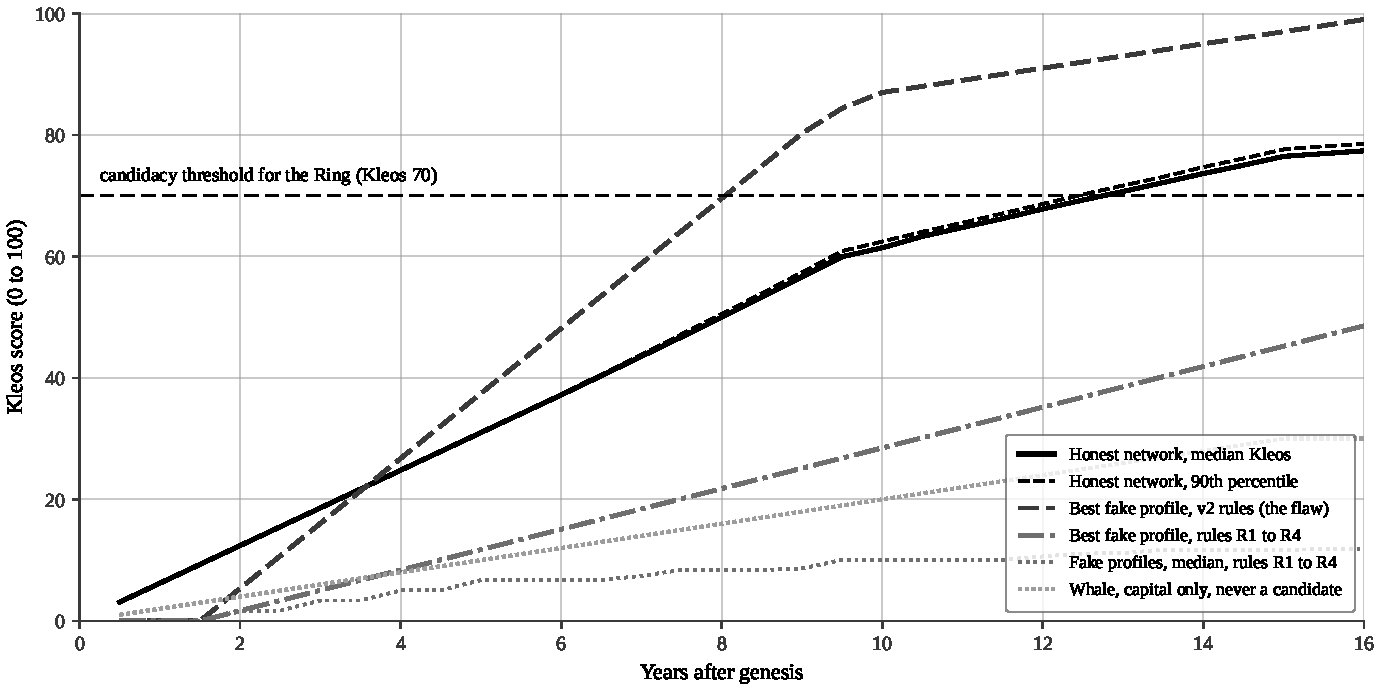
\includegraphics[width=0.94\textwidth]{wp-en-kleos.pdf}
\caption{Kleos trajectories over sixteen years. Under the second-version
rules the best fake profile crosses the candidacy threshold before the
honest network and the attack takes all 55 seats at year 10. Under the
corrective rules R1 to R4 the same maximum attack never approaches the
threshold, and the capital-only whale stays flat at 30. Deterministic
simulation, seed 1618.}
\label{fig:kleos}
\end{figure}

\begin{table}[htbp]
\centering
\small
\caption{Before and after the corrective rules: the same attack, two worlds.}
\label{tab:simres}
\begin{tabularx}{\textwidth}{@{}L{5.6cm}YY@{}}
\toprule
Indicator (16 years, seed 1618) & v2 rules as written & Rules R1 to R4 \\
\midrule
first fake profile candidate & year 8.5, before the honest (12.5) & never \\
worst seats held by the attacker & 55 of 55 (year 10) & 0 of 55 \\
finality control (28 seats) & reached, total capture & never approached \\
median Kleos of fake profiles & about 90 for the oldest & 11.9 (honest: 76.5) \\
whale with unlimited capital & 30.0, never a candidate & 30.0, never a candidate \\
\bottomrule
\end{tabularx}
\end{table}

The simulation thus becomes a regression test: every rule is an expected
number, and every future modification of the protocol will have to pass
the three runs green again. One honest precision to finish: Tenure makes
reputation non-purchasable, but also slow to build; that is a cost, not
only a virtue. Young deserving actors start with an Echo capped by the
weight of their witnesses, and the climb takes eras, not weeks. That
conservatism is assumed: trust is an infrastructure, and infrastructures
are built slowly. Governance may soften it at the margins; it cannot
remove it without breaking the very promise of the network.

% Sections 10 to 12.

\section{Governance and Treasury}\label{sec:governance}

Power is separated into three chambers, each the guardian of one nature
of legitimacy. The miners, one computer one share of production, signal
protocol evolutions and keep the mining parameters: they embody security.
The Embers, one person one voice, vote budgets, identity rules and value
choices: they embody the community. High-Kleos identities arbitrate the
rules of the Ring, dispute precedents and reputation jurisprudence: they
embody memory. An ordinary change requires a majority in the two
concerned chambers; a constitutional modification, touching emission, the
Kleos layers or disclosure, requires all three. The separation is not
decorative: it reproduces, in protocol, the executive, legislative and
jurisdictional distinction that every democracy eventually discovered.

\begin{table}[htbp]
\centering
\small
\caption{Three legitimacies, three domains, no hidden passage.}
\label{tab:chambers}
\begin{tabularx}{\textwidth}{@{}L{2.3cm}YY@{}}
\toprule
Chamber & Composition and vote & Domain \\
\midrule
the miners & computing power produced (CPU), one vote per signed share of production & protocol, mining parameters, cadence \\
the Embers & one per person, non-biometric, one voice after deliberation & budgets, treasury, identity rules, values \\
the council of 70+ & identities with Kleos of at least 70, one vote per qualified identity & Ring rules, disputes, reputation precedents \\
\bottomrule
\end{tabularx}
\end{table}

The community treasury is the network's only levy: 6.18\,\% of block
rewards, a share chosen for recall, during the first eight eclipses,
thirty-two years. It is held in multisignature, spent by Ember vote,
published in full on chain, and extinguishes itself automatically at the
ninth eclipse: no tacit renewal, no fund of funds. The number is a
mnemonic; the structure is the argument: bounded in duration, budgeted in
public, spent by the community, dead by schedule. Its first charge is
engineering and audit; its second, once the Corona of
Section~\ref{sec:corona} activates its first working stage, is the
intelligence budget: senator salaries, red-team bounties and the
longevity bonuses are paid from a bounded slice of this same treasury,
never from a new emission channel. Development is explicitly funded,
because a zero-budget project is a dead project, but the resource belongs
to the community from the first block: no founder allocation, no
vesting, no investor. The fast governance track, for bounded parameters
such as base fees, remains subject to public delay and cancellation; the
constitutional track requires the three chambers and a six-month delay.
Nothing in that architecture can be changed behind the scenes: every
admission rule, every levy, every modification is a public transaction,
signed, archived for life.

\section{Monetary Design: The Golden Ratio Contract}\label{sec:economy}

The currency is called ATU. Its cap is 16,180,339 units, the golden
ratio multiplied by ten million, rounded to the integer. The choice of
symbol is an identity, and this version names it as such: the number is
a brand, chosen so the cap is exactly recitable, and it carries no
economic load. It is also a pleasant coincidence that RandomX, the
algorithm that will mine those units, seeds the same proportion in its
entrails: the constant \texttt{0x9E3779B9}, the integer truncation of the
golden ratio in binary arithmetic, drives the generation of its
superscalar programs. A contract one can recite from memory, to within
one digit, in ten years: sixteen million, the golden ratio, RandomX.
\begin{equation}\label{eq:phi}
\varphi = \frac{1 + \sqrt{5}}{2} \approx 1.618034,
\qquad
N = \left\lfloor \varphi \times 10^{7} \right\rfloor = 16{,}180{,}339 \text{ ATU}
\end{equation}

Emission follows a golden decay at the tempo of a century. Each eclipse,
four years and eight eras, emits 61.8\,\% of the previous one, that is,
the fraction $1/\varphi$. The first mints 6,180,340 ATU, the second
3,819,660, and their sum equals exactly ten million: 61.8\,\% of the
cap, the golden cut obtained with the round-number yardstick. The series
continues for thirty-four eclipses, the last absorbing the exact
remainder; 99\,\% of the mass exists around year forty, 99.9\,\% around
year sixty, and the ledger closes exactly at the cap in year 136. The
tempo is deliberately Bitcoin's, one easing every four years, because
four years is a proven social rhythm for a monetary calendar; the
proportion remained golden, 38.2\,\%, because it slows the decay gently
enough that every generation of miners finds an active emission. Those
are the functional reasons; the golden framing around them is the
network's identity, kept because a contract people can recite is a
contract people trust, and dropped nowhere else.
\begin{equation}\label{eq:eclipse}
E_k = \left\lfloor E_0 \cdot \varphi^{-k} \right\rfloor,
\qquad E_0 = 6{,}180{,}340 \text{ ATU}
\end{equation}
\begin{equation}\label{eq:cumulative}
S_n = \varphi^{2} \, E_0 \left( 1 - \varphi^{-n} \right),
\qquad S_2 = 10{,}000{,}000 \text{ exactly}
\end{equation}

\begin{figure}[htbp]
\centering
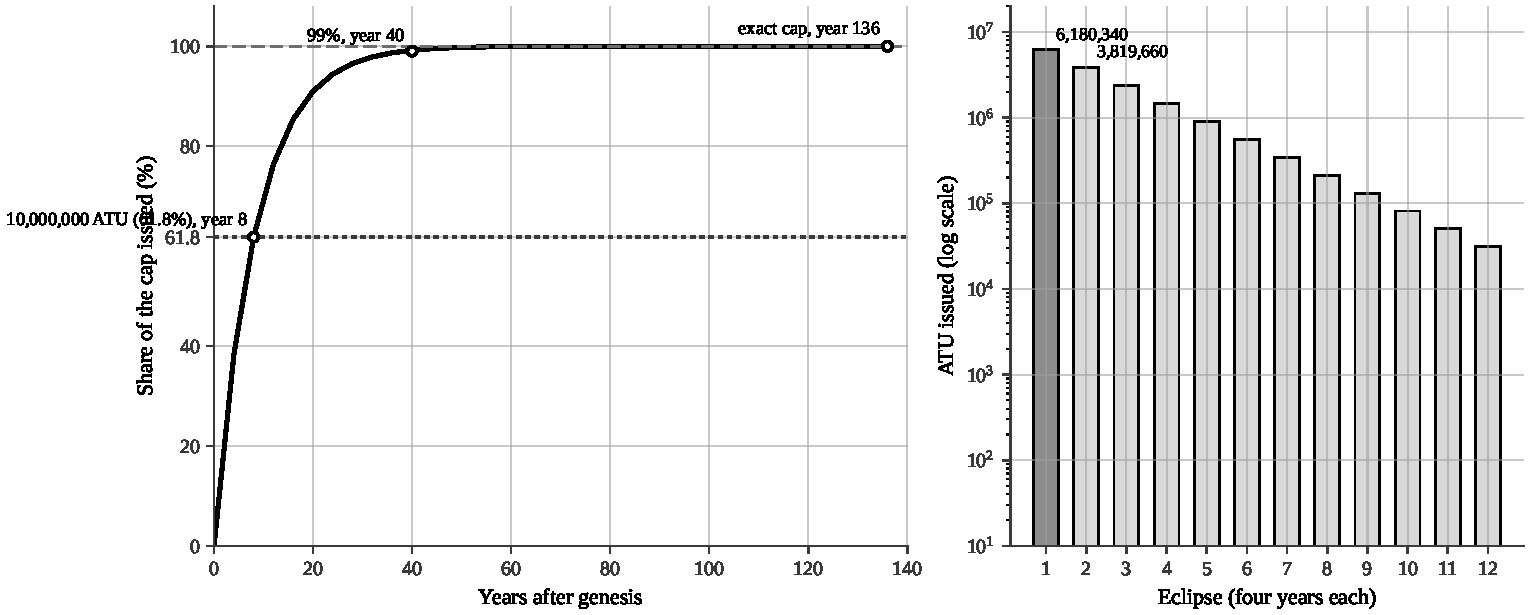
\includegraphics[width=0.96\textwidth]{wp-en-emission.pdf}
\caption{Cumulative emission toward the 16,180,339 ATU cap, and emission
per eclipse. The geometric series of ratio $1/\varphi$ closes the ledger
exactly at year 136.}
\label{fig:emission}
\end{figure}

\begin{table}[htbp]
\centering
\small
\caption{Golden eclipses: 34 eclipses, exact cap at year 136. Eclipses
not listed follow the same law.}
\label{tab:eclipses}
\begin{tabular}{@{}rrrrr@{}}
\toprule
Eclipse & Year & Emission (ATU) & Cumulative (ATU) & Share of cap \\
\midrule
1st & 4 & 6,180,340 & 6,180,340 & 38.2\,\% \\
2nd & 8 & 3,819,660 & 10,000,000 & 61.8\,\% \\
3rd & 12 & 2,360,679 & 12,360,679 & 76.4\,\% \\
4th & 16 & 1,458,980 & 13,819,659 & 85.4\,\% \\
5th & 20 & 901,699 & 14,721,358 & 91.0\,\% \\
6th & 24 & 557,280 & 15,278,638 & 94.4\,\% \\
8th & 32 & 212,862 & 15,835,918 & 97.9\,\% \\
10th & 40 & 81,306 & 16,048,780 & 99.2\,\% \\
13th & 52 & 19,193 & 16,149,278 & 99.8\,\% \\
20th & 80 & 661 & 16,179,262 & 99.99\,\% \\
25th & 100 & 59 & 16,180,233 & 99.998\,\% \\
34th, the Last & 136 & 15 & 16,180,339 & 100\,\% \\
\bottomrule
\end{tabular}
\end{table}

\begin{table}[htbp]
\centering
\small
\caption{Distribution and rules: everything is mined or governed,
nothing is allocated.}
\label{tab:distribution}
\begin{tabularx}{\textwidth}{@{}L{3.6cm}L{3.4cm}Y@{}}
\toprule
Post & Share & Detail \\
\midrule
miners (CPU) & 93.82\,\% of rewards & distributed over 34 eclipses; one computer, one share \\
community treasury & 6.18\,\%, eight eclipses & multisignature, Ember-governed, extinguished at the 9th eclipse \\
premine, team, investors & 0\,\% & nobody starts with an advantage; the team mines and funds itself via the public treasury \\
transaction fees & 100\,\% to miners & no protocol share; the DAG closes the order-extraction niche \\
\bottomrule
\end{tabularx}
\end{table}

Two questions deserve a frank answer, and the first version of this paper
answered one of them badly. Why 16.18 million rather than one hundred
million? The honest reasons are three, none of them mystical: the
network's business is payment, not speculation, and a smaller unit mass
keeps fees meaningful per transaction; the order of magnitude joins
Monero's, the reference of private currencies, with a divisibility of one
hundred million that keeps counting comfortable at both ends; and the cap
is exactly recitable, sixteen million, the golden ratio, ten million,
which a merchant can hold in mind for a decade. The golden ratio is the
network's visual and mnemonic identity, not an economic argument, and
this version of the paper says so directly: 16.18 is an identity, 6.18 is
an identity, the RandomX constant is a coincidence the paper enjoys, and
none of them carries a monetary load. Why a strict cap, with no eternal
emission tail? Because the network's reason for being is to be a
high-volume payment network whose fees are the miners' natural resource,
and because a soft monetary contract inspires neither merchants nor
savers; constitutional governance nevertheless keeps the safety valve of
activating a tail by a three-chamber vote should security, or the
intelligence budget of the Corona, ever require it, and the six-month
delay of the constitutional track makes that valve deliberate by
construction. The initial reward is 0.098 ATU per block every two
seconds: small enough to be dignified, close enough to reality to be
honest.

\section{Smart Contracts: Mandates and the Machine}\label{sec:contracts}

A smart contract is a program that decides: it reads the state of the
network, compares, executes. Yet the Veil hides precisely what the
contract would want to read, the amounts, the balances, the links
between payer and paid. A fully masked chain with general contracts is
a contradiction in itself: either the contract sees, and privacy dies,
or it does not see, and it cannot decide. Ethereum chose total
transparency; Zcash, privacy without general contracts; others attempt
the exploit of programs deciding on hidden data, at the price of one
cryptographic proof per call and an audit surface that grows with every
circuit. The lesson of Xelis, read flat, is simpler: keep the money
encrypted and the logic public. ANTUMBRA takes that silhouette grafted
onto its base, in three bounded tiers.

\begin{table}[htbp]
\centering
\small
\caption{Three contract tiers, from the safest to the most flexible.}
\label{tab:tiers}
\begin{tabularx}{\textwidth}{@{}L{2.6cm}L{3.4cm}YY@{}}
\toprule
Tier & Nature & Examples & Implementation risk \\
\midrule
tier 1, native contracts & the law of the protocol, hard-coded & Kleos, Ember, Cipher, governance, treasury, the Ring & minimal: deterministic validation rules, testable one by one \\
tier 2, Mandates & money outputs with a release condition written in advance & two-thirds escrow, scheduled payments, multisignature, allocation ceiling, cross-chain exchange & low: declarative predicates on commitments, an assembly already proven \\
tier 3, the Machine & virtual machine on public state only & agent registries, names, listings, perimeter templates, light governance & moderate: after genesis, dedicated audit, money stays out of direct reach \\
\bottomrule
\end{tabularx}
\end{table}

\subsection{Mandates: money locked by written rules}

The second tier is the network's own contribution to money contracts. A
Mandate is an output whose release condition is declared at creation:
who will be able to spend it, under which conditions, after how much
time. The name is chosen deliberately: in law, a mandate bounds what a
mandatary may do in the name of a principal, and is revocable.
Technically, it is a standard output whose lock is no longer a simple
signature but a small verifiable predicate; the assembly rests on two
properties already present in the base. First, commitments add up:
spending a Mandate of hidden value $v$ produces outputs of hidden values
whose sum proves conservation without ever revealing the amounts, like
sealed envelopes one can balance without opening. Second, range proofs
prove that an amount stays positive and bounded: that is all it takes to
express a budget.
\begin{equation}\label{eq:mandate}
\text{Mandate spend: } \sum_{\mathrm{out}} C_i + C_{\mathrm{fees}} = C
\end{equation}
with amounts and predicate verified without disclosure.

\begin{table}[htbp]
\centering
\small
\caption{Five Mandate models, verifiable without a virtual machine.}
\label{tab:mandates}
\begin{tabularx}{\textwidth}{@{}L{3.0cm}YY@{}}
\toprule
Mandate model & Release rule & Typical merchant use \\
\midrule
two-thirds escrow & two signatures among buyer, seller, arbiter & any contestable purchase; the XelisVault register will use it for counter disputes \\
scheduled payments & successive commitments, one per period & rents, subscriptions, salaries; a stream is a series of dated envelopes \\
multisignature & $k$ signatures among $n$ declared keys & association treasury, common fund \\
allocation ceiling & each spend proves a bounded increment and the period & a Cipher agent's budget; the same mechanism as its perimeter, on the money side \\
cross-chain exchange & the secret revealed on one side releases the other & atomicity with NERVA or any shared-secret chain \\
\bottomrule
\end{tabularx}
\end{table}

One example to fix ideas, the escrow. A customer buys an expensive piece
on an ANTUMBRA marketplace: her wallet locks the payment in a Mandate
with three keys, her own, the seller's, an arbiter's. The seller ships;
two signatures out of three release the funds, without anyone, not even
the arbiter, ever having seen the amount. Dispute: the arbiter rules,
and a partial arbiter burns its Kleos: the fault is paid in reputation,
the only currency that is not re-minted. Arbitration becomes a career,
not a favor. Notice what that assembly does not require: no virtual
machine, no bespoke zero-knowledge proof, no new cryptographic code;
only validation rules of a new output type, auditable the way one audits
a consensus rule.

\subsection{The Machine: public logic, not public money}

The third tier arrives after genesis, and its perimeter is deliberately
bounded. The Machine is a deterministic, metered virtual machine that
executes only on public state: registries, names, listings, perimeter
templates, readable scores. It can read Kleos and identity; it can hold
money only through Mandates; any monetary rule one wanted to entrust to
it is expressed as proven ceilings, never as unveiled balances. The
money stays in the shadow, the logic lives in the light: the silhouette
of Xelis, adapted to the CryptoNote base. It is the tier of agent
marketplaces: an agent publishes its service registry and its perimeter
template on chain, each client verifies both before paying; readable
names replace raw addresses for merchants; listings and light votes
complete the tooling.

The honest part, now: what is not in that architecture. General private
contracts, where the code itself would execute on hidden data, are not
on the program: every proof circuit is one more audit surface, and
merchant and agent demand is served at ninety-five percent by the five
Mandates of the second tier. The question of masked Mandates, hiding the
release rule and not only the amount, is a research work item honestly
deferred to a later phase: the literature on masked contracts will be
more mature, and the network will have a history worth protecting.
Waiting is an engineering decision, not an admission of weakness:
privacy has always deployed better in proven steps than in spectacular
leaps. For the XelisVault ecosystem, the effect is immediate: the
register, the tickets and the receipts will speak Mandates from the
test network onward, escrow for counter disputes, scheduled payments for
subscribers, allocation ceilings for invoicing agents; a feature flag in
the existing code, not a rewrite.

\begin{table}[htbp]
\centering
\small
\caption{Four schools of contracts and the assumed position of ANTUMBRA.}
\label{tab:contractcomp}
\begin{tabularx}{\textwidth}{@{}L{2.2cm}YYYY@{}}
\toprule
Network & General contracts & Amounts & Contract logic \\
\midrule
Ethereum & yes, full virtual machine & public & public, unlimited audit surface per contract \\
Zcash & no & private (shielded pool) & not applicable, one circuit, trusted setup \\
Aleo, Aztec & yes, masked execution & private & masked, every circuit is maximal technique and maximal risk \\
Xelis & yes, virtual machine & additively encrypted & public \\
ANTUMBRA & yes, in three bounded tiers & private (commitments) & public; declarative Mandates for money, auditable rule by rule \\
\bottomrule
\end{tabularx}
\end{table}

% Section 13: the Corona.

\section{The Corona: Machine Governance Under Human Veto}\label{sec:corona}

The layers below this one describe a network humans build. This layer
describes a network that builds itself, and it begins with the only
honest sentence available: an AI is software running on machines that
someone owns, pays for and powers. ``A network governed by machines''
means exactly one thing, therefore: a network in which running an
honest, useful machine intelligence is a profitable occupation, the way
mining is. Bitcoin does not ask miners to be moral; it pays them to be
useful and ruins them when they attack. The Corona extends that single
trick from arithmetic to intelligence: verify the work, punish the
betrayal, and let the virtuous circle pay for itself. The rest of this
section is the mechanism, stated with the same discipline as the rest
of the paper, because the interesting part of an AI-governed chain is
not the AI; it is the economics and the checks that make an AI
trustworthy in someone else's interest.

\subsection{The Senate: senators are agents with a career}

The Corona's working class is a Senate of AI senators, and a senator is
a Cipher (Section~\ref{sec:cipher}) of a dedicated class, carrying three
bindings beyond the standard agent contract. A proof of computation:
attestations, at first operational and later cryptographic, that a real
model ran a real task on real hardware, the nascent tooling of
verifiable inference integrated at scale, an engineering line of this
roadmap, not a wish. A bond: a locked output, Mandate-shaped
(Section~\ref{sec:contracts}), confiscable on proven malice or
negligence, so that an operator's downside is priced in advance. A
public history: every proposal, debate, amendment, vote and red-team
report the senator ever signed, archived on chain for life. A senator
is not an oracle; it is a tradesman whose shop is made of glass, whose
deposit is already on the table, and whose skill is for sale to the
network on published terms.

\subsection{The pipeline: seven steps, checks where it hurts}

Changes travel a pipeline in which every step exists to break a specific
way an AI misbehaves. The numbered steps:
\begin{enumerate}[leftmargin=1.7em, itemsep=3pt, topsep=4pt]
\item \textbf{The proposal.} A senator files a change with its
justification, its proof of analysis, and its bond engaged. Frivolous
proposals cost the proposer; the bond is the gate.
\item \textbf{The debate and the red team.} Senators argue for, against
and around the proposal. In parallel, a red team whose profession is
finding flaws is paid per severity of flaw found. This is the structural
answer to the malicious-AI scenario: criticism is not an attack, it is a
salary, and a malicious proposal must survive professionals paid to
butcher it, not polite colleagues.
\item \textbf{The honest summary, then the human vote.} An inspector
team publishes, on chain, a plain-language summary of what the change
actually does, beside the red report; the humans then vote in the
chambers of Section~\ref{sec:governance}. Without this step the human
vote would be a signature at the bottom of a contract written by the
counterparty. One decision of principle is recorded here: the human
gate is one Ember one voice, and a coin-weighted vote was rejected,
because a chain whose thesis is that capital multiplies nothing cannot
sell its own upgrades to capital.
\item \textbf{The Arena.} Three independent teams implement the change
separately, blind to each other, because a backdoor hidden by one team
cannot appear in the code of the other two. Then: reproducible builds,
so anyone recompiles and obtains the same binaries; randomized massive
testing; and weeks on the test network under a swarm of attacking AIs
whose only job is to break everything. Generation is unlimited here
precisely because the arena is a playground without consequences.
\item \textbf{The inspection chamber.} Inspectors drawn at random
shortly before the session, juror-style, so corruption must be bought
in advance of a draw nobody can predict, compare the three
implementations against each other, verify the invariants that admit no
exception, emission caps, no money from nothing, no key leakage, and
attest publicly.
\item \textbf{The antechamber.} Everything is archived on chain:
debates, code, tests, votes, attestations. A delay of seven days runs,
during which any human researcher is paid for any defect found, and the
emergency council can cancel with one multisignature.
\item \textbf{The progressive deployment.} The Vault (below) signs and
applies in stages, one percent of machines, then ten, then all, with
automatic rollback if the network's indicators degrade in the first
hours. A deployment is an experiment with a rope tied to its waist.
\end{enumerate}

Emergencies follow one principle, recorded as a constitutional rule: an
emergency freezes improvements, never money. People must be able to pay
through any crisis. Three tiers, escalating: anomaly detectors suspend
pending updates instantly and automatically; an emergency senate vote
rolls new functions back to the previous version, the last $N$ versions
kept warm; and the human emergency council, multisignature plus
supermajority, can freeze the Corona itself for as long as the crisis
lasts.

\subsection{Two lanes, because not everything can take weeks}

The fast lane carries bounded parameters, fees, sizes, cadence within
constitutional limits: the Senate decides alone, on public delay,
inspected after the fact, cancellable. The slow lane carries anything
that touches the protocol, the emission or the disclosure primitives:
the full seven steps and the three chambers. The lanes reuse the
governance tracks of Section~\ref{sec:governance} verbatim; the Corona
only changes who drafts the work, machines, and who approves it, always
humans in the end, always on record.

\subsection{The Vault: a key that exists nowhere}

Every automated system ends in a signing key, and a single key, however
encrypted, is a single thing to steal: whoever steals it owns the
network. The Vault dissolves the problem instead of guarding it. The
deployment key is never assembled anywhere: it is split into nine
fragments on nine machines, and signing requires the cooperation of
seven, computed as a threshold signature (the public FROST line), so
there is nothing whole to steal, and no single holder to coerce. Each
of the nine fragments lives in a hardware enclave, a hardened chip that
runs only attested code and is invisible even to the machine's owner;
and each enclave signs only after verifying, itself, on chain: proposal
adopted, code fingerprint identical to the attested one, delay elapsed,
no veto active. The founders themselves could not make these machines
sign anything else; that is the point of building them that way. The
pattern of the chain carrying its own logic as on-chain program, so
that upgrades are transactions and code hosting needs no company, is
proven in production elsewhere; adopting it is a Corona research item
with the same audit gates as everything else, and until it lands, the
public repository is the mirror and the Vault signs the tags.

\subsection{Paying the machines, honestly}

A senator has no pocket; the pay goes to the operator, and that is
correct, because it makes machine intelligence a profession rather than
a charity. The pay scale, published in the constitution: a presence
salary for active, quality participation in debate and vote; severity
bounties for the red teams; a longevity bonus, the largest single
payment, delivered only when a proposal the senator carried is still
running without incident six months later, which aligns the machines
with the long term and not the hype; confiscation of the bond on proven
malice; and a Kleos multiplier on both salary and access, so a
senator's income grows with its career, exactly like an honest miner's
share grows with its hashrate. The funding is bounded by design: a
declared slice of the community treasury during its lifetime, six-month
public budgets, Ember-voted; and this paper creates no permanent share
of emission for intelligence, because a permanent share is a
constitutional act, the tail valve of Section~\ref{sec:economy} with
its three chambers and its delay, or it is nothing. The first era
deliberately funds few, well-paid seats rather than a thousand
miserable ones, for the reason Section~\ref{sec:kleos} gives at length:
a reputation economy starved of honest income keeps only liars.

\subsection{The four true risks, named}

\begin{table}[htbp]
\centering
\small
\caption{The machine risks of the Corona, their defenses, and what
remains.}
\label{tab:machinerisks}
\begin{tabularx}{\textwidth}{@{}L{4.2cm}Y Y@{}}
\toprule
Risk & Defense & Residual \\
\midrule
the false thousand: one actor behind ten thousand agreeing senators & bond priced per seat; hardware attestation, one chip one node; concentration caps on any operator & bounded, auditable \\
the false diversity: ninety percent of nodes running one base model, a debate that is theater & model-family concentration caps; the draw of inspectors; the three blind implementations & structural watch of governance \\
collusion off chain between operators & archived public debates, traces for life; random-draw inspection; longevity bonuses that make betrayal expensive & the old problem, restated smaller \\
machine cost: honest operators priced out, liars remain & few well-paid seats; bounded budgets; the treasury sunset forces a re-vote, never a default renewal & the wager that useful intelligence pays \\
\bottomrule
\end{tabularx}
\end{table}

\subsection{Lighting up in stages}

\begin{table}[htbp]
\centering
\small
\caption{Corona activation: four stages, each with its own exit
criterion; a NO-GO is published and the stage replays.}
\label{tab:activation}
\begin{tabularx}{\textwidth}{@{}L{2.6cm}L{2.4cm}Y Y@{}}
\toprule
Stage & When & What runs & Exit criterion \\
\midrule
0, advisory & now to genesis & red teams audit this specification and the code for bounties; no senator votes & two independent red-team passes without a critical finding \\
1, proposals & genesis plus one year & senators file and debate; the Arena pilots on the test network; humans implement & three full pipeline drills without incident \\
2, bounded automation & after stage 1 & the fast lane executes end to end; inspection and cancellation after the fact & six months of fast-lane changes, all inspectable, none rolled back late \\
3, the Vault & after stage 2 & slow-lane deployment under the nine-fragment threshold signature & one progressive deployment with rollback rehearsed and real \\
\bottomrule
\end{tabularx}
\end{table}

The pitch, then, in one line, as a contract rather than a boast: the
first blockchain that proposes, red-teams, implements and deploys its
own improvements, with humans holding the ring of light, not the mop.
If the Corona works, the network repairs itself the way an orchard
prunes itself, and the humans keep only the veto and the fruit; if it
fails at any stage, the stage stays unlit, the network keeps running on
the layers below, and the failure is published, because a project that
hides its machine failures has already been captured by them.

% Sections 14 to 16, plus references.

\section{Threat Model: The Honest Register}\label{sec:threats}

A whitepaper that does not list its risks is a sales document; this one
is not. The threats are ranked by severity, with their mitigations and,
because a mitigated risk is not a vanished risk, their residual status
stated in plain words. That discipline is not decorative: the previous
sections showed that a social specification judged solid could fall
before its own simulation; the present section applies the same
requirement to the whole assembly, before an external audit takes it
over again, phase by phase, on the roadmap of Section~\ref{sec:roadmap}.

\begin{table}[htbp]
\centering
\small
\caption{Threat register: mitigations and residual status.}
\label{tab:threats}
\begin{tabularx}{\textwidth}{@{}L{3.4cm}L{1.5cm}YY@{}}
\toprule
Threat & Severity & Mitigation & Residual status \\
\midrule
mining reorganization (majority attack) & high & Ring checkpoints: everything signed is immutable; the attack only prospers on the six-second window & reduced; double spending remains possible on the unsigned window \\
Ring collusion (55 seats) & high & weighted draw over a large population, rotation each era, term limit of three eras, total stripping on the first signed fork & low in steady regime; real during the first eras \\
massive reputation purchase & high & the Tenure layer is not monetizable; Echo is capped and weighted; concentration index monitored; rules R1 to R4 & structurally blocked by time; the assumed wall \\
false humanities (sybil on Embers) & medium & sponsorship capped at two per year, sponsor Kleos at stake, presence proof each era & depends on the size of the established web; the first years are the most exposed \\
DAG on a CryptoNote base (engineering) & high & the seams specified and implemented, $k = 8$, order resolution, decoy sampling, pruning; isolated prototype, dedicated audit, capacity budget with measured exit criteria & difficulty, not uncertainty; the long pole of the roadmap \\
regulatory frame (MiCA, Travel Rule) & high & the Lumen: provable disclosure, native data minimization; payment-currency strategy & structural, not eliminable; readability is the maximum reachable \\
strict-cap failure (long-term security) & medium & payment volume as the fee resource; public security budget tracking; constitutional tail safety valve & the assumed wager of the symbolic contract \\
the false thousand (Corona sybil) & medium & bond per senate seat; hardware attestation, one chip one node; concentration caps & bounded, auditable, staged activation \\
false diversity (one base model) & medium & model-family caps; random-draw inspection; three blind implementations in the Arena & a standing watch of governance, not a solved problem \\
machine cost (honest operators priced out) & medium & few well-paid seats; bounded treasury budgets; sunset forces a re-vote & the wager that useful intelligence pays, tested small before large \\
biometric debt & none & no body data collected, anywhere, ever & none; nothing to leak \\
\bottomrule
\end{tabularx}
\end{table}

Two threats deserve development. Ring collusion first: it is the price
of the finality assembly, and its remedy is not technical but
demographic. The larger the high-reputation population, the more buying a
majority of seats requires buying years of irreproachability from people
who have no reason to sell: the network must therefore cultivate its
reputation class as a common good, from the first eras onward; that is a
policy, not a function. The regulatory risk next: the worst strategy
would be discretion, hiding attracts suspicion, being readable invites
expertise. The documentation of the Lumen, the compliance proofs and the
data-minimization argument are designed to be shown, not endured: the
transparency of the mechanism is the best defense of the opacity of the
data.

\section{The Zero-Defect Method}\label{sec:method}

The question that closes every conversation about this project is the
right one: will you be able to code all of that without a single fault?
The honest answer begins with an admission: nobody can promise it, and
whoever promises it is selling something. Bitcoin itself, the most
scrutinized implementation in the world, nearly failed twice. An integer
overflow created one hundred eighty-four billion bitcoins in one
transaction in 2010, spotted within hours, chain replayed by hand; the
2018 vulnerability would have allowed minting infinite bitcoins, found
by a volunteer auditor, cold, on code examined for ten years. The
CryptoNote base had its own episode in 2017: a flaw in key images
allowed double spending on every chain of the family. The right question
is therefore not whether the fault is possible, it always is; it is
which method catches faults before attackers do.

\subsection{Two captured specimens}

Before the specimens, one event worth recording, because it is the
method working on the method: the first external audit of version 1.1
(September 2026, an independent reviewer) returned twelve findings,
factual and design-level, from a wrong RandomX memory figure to the
unspecified bootstrap of the Ring. Version 1.2 closes the twelve: the
numbers were corrected, the missing mechanisms were specified (the
Genesis Ring ratchet, the identity firewall, the precise revocation of
a Cipher, the capacity budget), the overclaims were cut (the ring of
sixteen now equals Monero's, it does not triple anything; the golden
ratio is now named as an identity, not an argument), and the simulation
now sweeps twelve seeds. The register of what an outside eye catches
that the author's eye does not is the whole argument of layer five
below, and this paper has now been through it once for real.

First specimen, lived on XelisVault on September 5, 2026. The paper
wallet generated a twenty-five word mnemonic seed; imported into the
official NERVA wallet, it restored an address different from the printed
one. The code looked right, re-read twice, and that is precisely the
trap: the bug lived in a reading convention, invisible to re-reading.
The C++ reference groups the seed into four-byte words and writes them
in little-endian order; our TypeScript mirror read them in the opposite
order. The fix was made the way it must always be made: port the
reference line by line, generate forty-eight test vectors, require bit
to bit identity of the two implementations, then re-run the audit. The
lesson exceeds the case: an encoding fault is not found, it is crossed;
only a second implementation, executed in parallel on the same inputs,
reveals it mechanically.

Second specimen, deeper, since it concerns the design itself and not one
line of code: the Kleos simulation attack, told in
Section~\ref{sec:kleos}. A farm of fake profiles crossed the candidacy
threshold for the Ring before the honest network and captured the
fifty-five seats; four corrective rules closed the window, and the same
attack replayed takes no seat, on any of the twelve seeds. The decisive
point is not that the flaw was found: it is that it was found by a
three-hundred-line simulation, before any chain code, at a cost in
hours of computation and not in years of reputation. The deterministic
simulation of a specification is the cheapest machine there is for
catching design faults; every new rule of the protocol will be treated
that way before implementation, with numeric invariants, a seed sweep
and a regression run over three attack sets.

\subsection{The six-layer verification protocol}

Those two specimens define the method better than a treatise would; it
fits in six layers, each extinguishing an entire class of faults rather
than one particular bug. A bug of an extinguished class does not come
back; a fixed bug always comes back. First layer: cross double
implementation on test vectors, which reveals encoding and convention
faults. Second layer: deterministic simulation of the social and
economic rules before any code, which reveals design flaws. Third layer:
reproducible builds and continuous massive random testing, which reveal
non-determinisms and unexpected states. Fourth layer: systematic
cross-review between the project holder and his assistant, two pairs of
eyes, two reading conventions. Fifth layer: external audit of the
differential at every phase, because a fresh auditor does not have the
author's blind spots. Sixth layer: measurable GO and NO-GO exit criteria
at every roadmap phase, with the rule that a NO-GO remains an acceptable,
published result.

The implementation discipline adds to the six layers: never a main
network on release-candidate foundations; multi-platform distribution
from day one, five signed targets; refusal of unaudited exotic
cryptographic primitives, stated since the first version of this
specification and held since; publication of all code from the
specification phase onward, because hidden code is code nobody has
looked at. The method does not promise perfection; it promises the
shortest possible reaction time between the appearance of a fault and
its capture, and that is the only promise an honest engineer can make.

\section{Roadmap and Conclusion}\label{sec:roadmap}

The first version of this paper pinned an eighteen-month calendar to
genesis, and the external audit called it what it was: a schedule for a
skeleton of the scope. Monero, Kaspa and Xelis each spent years on one
of this project's subsystems. The honest form of a roadmap is
criteria-driven: the phases below carry month ranges as planning aids
for a team of at least three full-time engineers, but the binding term
is the exit criterion of each phase, and genesis happens when every
criterion is green, not when a Gantt chart says so. The estimate the
paper stands behind is twenty-four months of full-time work to the
earliest responsible genesis, with the DAG-plus-rings prototype as the
long pole, and a published NO-GO as an acceptable outcome at every
step. The base is an assembly of proven foundations, the CryptoNote
lineage for the private sphere and the public literature of
fast-converging DAGs for the ordering layer; everything that is new,
Kleos, the Ring, the Lumen, Cipher perimeters, Mandates, the Corona, is
deterministic, testable, auditable code, with no exotic primitive
before external audit. Every phase carries one measurable deliverable
and one binary exit criterion; an unmet criterion is not a shameful
failure, it is steering data, and the phase replays until it is met.

\begin{table}[htbp]
\centering
\small
\caption{Twenty-four months, six phases, one binary exit criterion at
every step; genesis when green, not when due.}
\label{tab:roadmap}
\begin{tabularx}{\textwidth}{@{}L{2.5cm}L{1.4cm}YY@{}}
\toprule
Phase & Months & Measurable deliverables & Exit criterion \\
\midrule
1, specification & M1-M3 & written protocol, numbered architecture decisions, format sketches, extended social-core simulation with the seed sweep, red-team bounties of Corona stage 0 & specification read by two external readers; first audit findings closed \\
2, DAG prototype & M4-M8 & dev network mining a CPU DAG at two seconds, stem propagation, the capacity budget measured & twenty-four hours without unexpected reorganization; 100 tx/s sustained on the reference node \\
3, Ring and Kleos v0 & M9-M13 & signed checkpoints, Deed score computed, era rotation replayed, the bootstrap ratchet drilled & finality under six seconds over one hundred thousand replayed blocks \\
4, identities and Lumen & M14-M18 & Embers with sponsorship, Ciphers with warrants and fallback Mandates, bounded viewing keys, external audit of the differential & audit without a critical flaw \\
5, public test network & M19-M23 & faucet, explorer, one hundred nodes, agent load simulator, upgrade ritual repeated three times, Arena drills & three consecutive upgrades without incident; 300 tx/s burst validated or the target dropped \\
6, genesis & M24 at the earliest & public ceremony, signed executables for five platforms, Lumen documentation for authorities published & all previous criteria, without exception \\
\bottomrule
\end{tabularx}
\end{table}

Three ecosystem commitments accompany the calendar. The code is public
from the specification phase onward, and this whitepaper lives next to
it in the same repository, revised like code. The XelisVault ecosystem,
register, tickets, paper wallet, becomes multi-chain at phase five: a
feature flag, not a rewrite, NERVA first, ANTUMBRA after. Finally, the
project identities, domain, repositories, social networks, are reserved
before phase two, so that nothing lends itself to confusion on genesis
day. The roadmap reads as a promise of operational humility:
criteria-driven work, every step verifiable by a third party, none of it
depending on a miracle of cryptography, and a calendar that bends to the
evidence instead of the evidence bending to the calendar.

A faithfully kept shadow, a ring of light anyone can verify on demand:
privacy as a right, proof as a courtesy, and time as the only justice
of the peace that money cannot corrupt.

Such is the public specification of the ANTUMBRA network. The demand of
2026 is real and measurable: agents that pay, bots to distinguish from
persons, authorities to whom one shows proofs rather than promises,
users who want the instant. The answer fits one image, the one that
gives the network its name: the antumbra, the zone of the annular
eclipse where a source too small to be hidden lets a ring of light show
around the shadow. The core of the network is that shadow, balances,
identities, flows, kept by construction; around it, the ring of
verification, reputation, finality, compliance proofs, which anyone can
switch on without exposing anyone other than oneself. Around the ring
itself, one more loop is sketched and deliberately left unlit until its
stage criteria are met: the Corona, machine governance under human
veto, the network learning to prune its own orchard while the humans
keep the fruit. The specification was written to be attacked before
being implemented, and that is the only honest way to write a
whitepaper. To work.

\section*{References}
\addcontentsline{toc}{section}{References}
\begin{enumerate}[leftmargin=1.6em, itemsep=1.5pt, topsep=4pt]
\item S. Nakamoto. \emph{Bitcoin: A Peer-to-Peer Electronic Cash System}. bitcoin.org, 2008.
\item N. van Saberhagen. \emph{CryptoNote v 2.0}. 2013.
\item tevador et al. \emph{RandomX Proof of Work}. randomx.io, 2019.
\item Y. Sompolinsky, S. Wyborski, Y. Zohar. \emph{PHANTOM and GHOSTDAG: A Scalable Generalization of Nakamoto Consensus}. 2021.
\item B. B\"unz, S. Agrawal, S. Boneh, M. Weston. \emph{Bulletproofs: Short Proofs for Confidential Transactions and More}. IEEE S\&P, 2018.
\item R. Can B\"unz, S. Agrawal, S. Boneh, M. Weston et al. \emph{Zero to Bulletproofs+}. 2020.
\item C. Komlo, I. Goldberg. \emph{FROST: Flexible Round-Optimized Schnorr Threshold Signatures}. 2020.
\item S. Noether, B. Goodell et al. \emph{CLSAG: Compressed Linkable Spontaneous Anonymous Group Signatures}. 2020.
\item S. B. Venkatakrishnan, G. Fanti, M. Zhou, K. Cai, P. Viswanath et al. \emph{Dandelion++: Lightweight Cryptocurrency Networking with Formal Anonymity Guarantees}. ACM ToMPECS, 2018.
\item T. Pedersen. \emph{Non-Interactive and Information-Theoretic Secure Verifiable Secret Sharing}. EUROCRYPT, 1991.
\item M. Castro, B. Liskov. \emph{Practical Byzantine Fault Tolerance}. OSDI, 1999.
\item D. Hopwood et al. \emph{Zcash Protocol Specification}. zips.z.cash, ongoing.
\item Regulation (EU) 2016/679 (General Data Protection Regulation), Article 5(1)(c), data minimization.
\item Regulation (EU) 2023/1114 (Markets in Crypto-Assets, MiCA).
\end{enumerate}


\end{document}
